% ============================ Enrico Ribiani 16-03-2021 ====================================================================
% Base per i documenti  
\documentclass[12pt]{article}
% ------------ pacchetti necessari ----------------
\usepackage[a4paper, total={6in, 8in},margin=1in]{geometry} % formattazione decente della pagina
%\usepackage{graphicx}                            % need for figure
\usepackage{amsmath}
\usepackage{amsfonts}                            % if you want the fonts
\usepackage{amssymb}                             % if you want extra symbols
%\usepackage{graphicx}  
\renewcommand{\figurename}{Figure}  
\renewcommand{\contentsname}{Index}                        % need for figures
\usepackage{mathptmx}
\usepackage{float}                               % serve per mettere tabelle e immagini dove si vuole 
\usepackage[utf8]{inputenc}
\usepackage{textcomp}
\usepackage[hang,flushmargin,bottom]{footmisc}   % footnote format
\usepackage{fancyhdr, lastpage}
\usepackage{titlesec}
\usepackage[table,dvipsnames]{xcolor}
%\pagestyle{fancy}
%\renewcommand{\headrulewidth}{0pt}
%\renewcommand*\contentsname{Indice}
\titleformat{\section}{\normalsize\bfseries}{\thesection.}{1em}{}	% required for heading numbering style
\titleformat*{\section}{\Large\bfseries}
\titleformat*{\subsection}{\large\bfseries}
%\usepackage{siunitx}
%\usepackage{tikz}
\usepackage{circuitikz}
%\usepackage[siunitx]{circuitikz}
\usepackage{multirow}
\usepackage{tikz}
\usepackage{amsmath}
\usepackage{shorttoc}
\usetikzlibrary{angles,quotes}
\usepackage{placeins}

\usepackage{wasysym}
%===================links=================
\usepackage{hyperref}
\hypersetup{
    colorlinks=true,
    linkcolor=darkgray,
    filecolor=Green,      
    urlcolor=Cyan,
    pdftitle={SAMPLE},
    pdfpagemode=FullScreen,
    }

\usepackage{graphicx}
%\usepackage{caption}
\usepackage{subcaption}

%===================inizio pagina del titolo=================
\begin{document}
\pagenumbering{gobble}
\begin{titlepage}
	\begin{center}
		% ------------------ inizio immagine logo ----------
		\begin{figure}
			\centering
			
\includegraphics[scale=1.2]{~/Documenti/latec/logo.png}
			\label{fig:logo}
		\end{figure}
		% ------------------ fine immagine logo ----------
		% ------------------ fine immagine logo ----------
		-------------------------------------------------------------------------------------\\
		\vspace{2\baselineskip}
		\large $5^a$AUB\\
		\large Enrico Ribiani\\
		\large Nicolò Cellana\\
		\large Marco Ciola\\


		\vfill

		\Huge{\textbf{Photovoltaic panels measures}}\\
		\vfill

		\LARGE{$5^{th}$ report}\\
		\vfill
		\large{19-05-2023}
	\end{center}
	%=============== fine pagina titolo ===============
\end{titlepage}
\tableofcontents
\newpage
\pagenumbering{arabic}
\setcounter{page}{1}
\section{Introduction}
This report will illustrate the laboratory experience, carried out on 12 May 2023, focused on the study of
photovoltaic panels.\\
The collection of data took place inside the courtyard of the ITT Buonarroti (TN), during the
afternoon with suitable weather conditions,direct sun exposure, positioning the panels appropriately with an
inclination of approximately 37° facing northwest.\\
We underline how the duration of the collection of the values could slightly compromise the reliability of
the measurements, this is mainly due to the variable exposure conditions of the panels to solar radiation
over time and the variation of temperature of the panels that reached 44°C starting from around 28°C.\\
The report also contains the analisys of the data collected, the power output and an approximative extimation
of the radiation.\\
PV cells are electrically connected in a module. PV panels vary in size and in the amount of electricity they can produce. PV panel electricity generating capacity increases with the number of cells in the panel or in the surface area of the panel. PV panels can be connected in groups to form a PV array.
Photovoltaic cells generate direct current (DC) electricity. Nearly all electricity is supplied as
alternating current (AC) in transmission and distribution systems. Devices called inverters are used to
convert the DC to AC.\\
PV cells and panels will produce the most electricity when they are directly facing the sun.\\
Most PV systems have panels in a fixed position that are usually facing directly south in the northern
hemisphere—directly north in the southern hemisphere, and at an angle that optimizes the physical
performance of the system.\\
The maximum current is obtained in the short circuit configuration and the maximum voltage is obtained
with the open circuit configuration.\\
Connecting the rheostats in series leads to a higher tension and a lower current and viceversa for the parallel.\\

\section{Pv panels theory}
\begin{figure}[!ht]
	\centering
	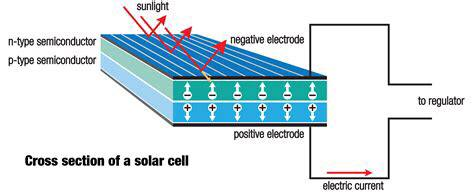
\includegraphics[scale=0.4]{theory.jpg}
\end{figure}
\noindent
The main component of a PV Panel are the PV cells, a photovoltaic cell is a nonmechanical device that
converts sunlight directly into electricity.\\
Sunlight is composed of photons, or particles of solar energy.
These photons contain varying amounts of energy, called Quanta, that correspond to the different wavelengths
of the solar spectrum. \\
A PV cell is made of semiconductor material.\\
When photons strike a PV cell, they may reflect off the cell,
pass through the cell, or be absorbed by the semiconductor material. Only the absorbed photons provide
energy to generate electricity. When the semiconductor material absorbs enough sunlight, electrons are
dislodged from the material's atoms. Special treatment of the material surface during manufacturing makes
the upper surface of the cell more "receptive" to the free electrons so that the electrons naturally
migrate to the surface of the cell.\\
The movement of electrons, each carrying a negative charge, toward the front surface of the solar
photovoltaic cell creates an imbalance of electrical charge between the cell's front and back surfaces.\\
This imbalance, in turn, creates a voltage potential like the negative and positive terminals of a battery.\\
Electrical conductors on the cell absorb the electrons. When the conductors are connected in an electrical circuit to an external load,
such as a battery, electricity flows through the circuit.\\
\section{Request}
The objective of this activity was to survey the characteristics of three photovoltaic panels made with different
technologies and from their comparison derive an estimate of the incident energy.\\
In order to achieve this we collected the current and the tension generated by the three panels and write
the values in Excell tables.\\
Using the voltamperometric measurements collected under the same condition and in different load configurations we were asked to trace the graph of the
panels characteristics.\\
Using the graphs we traced and the ones in the datasheets we are requested to estimate the radiation on the
panels.\\
\section{Wiring diagrams}
\begin{figure}[ht]
	\centering
	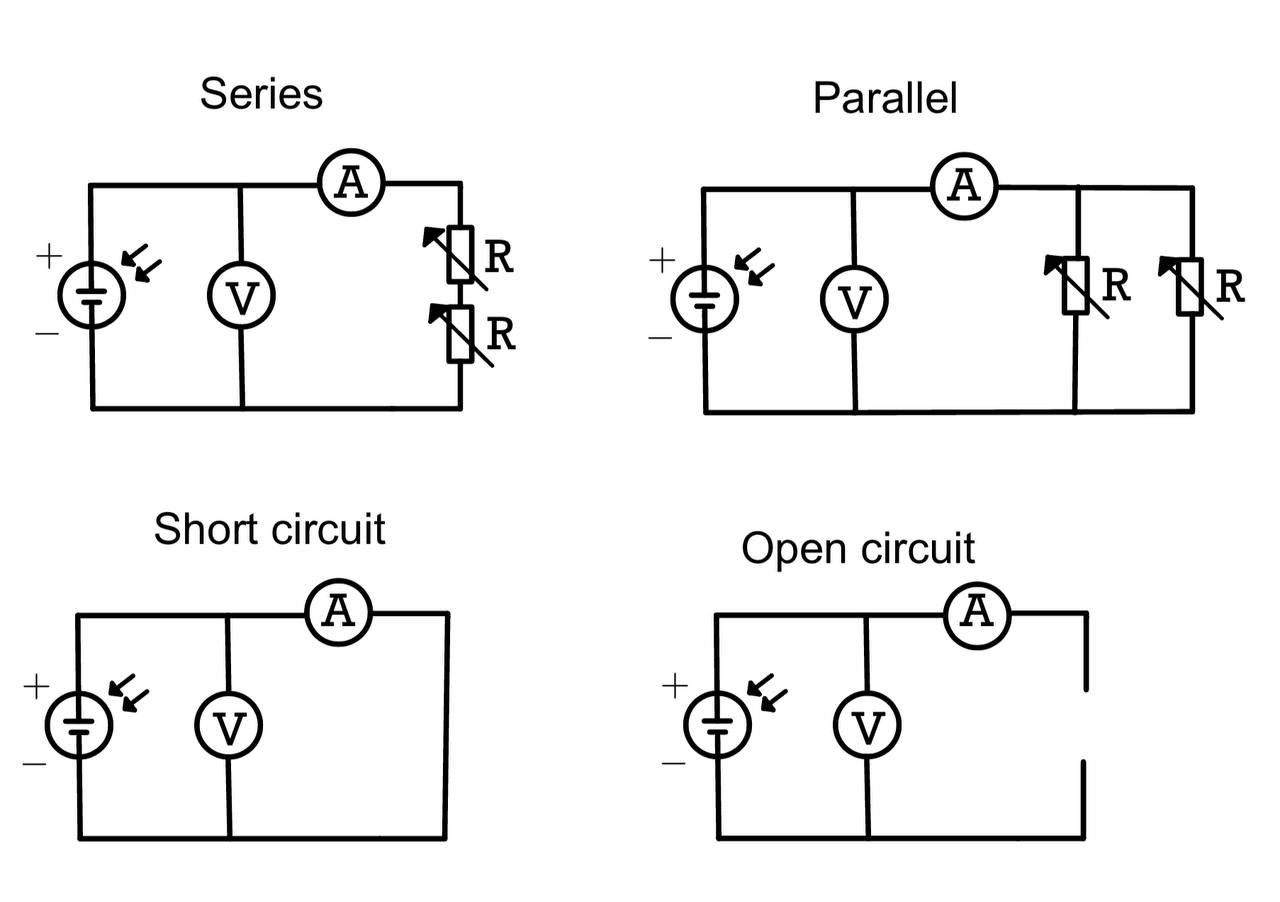
\includegraphics[scale=0.2]{schema.jpg}
\end{figure}
\newpage
\subsection{Equipment}
\begin{itemize}
	\item Connection Wires
	\item Benq PM245P00
	\item Panda 60 cells
	\item Sharp NA-E135L5 series
	\item 2x Rheostat  $200\Omega$ and 2,5A maximum
	\item 2x Multimeter
\end{itemize}
All the equipment is certificated and used in optimal condition.\\
\section{Procedure}
First of all even before starting the wiring process we calcuted the max current with the
full resistance of the rheostat and the maximum current of the panels and we chose to put the ammeter in
DC current with the maximum value mesurable at 20A.\\
For every panel we first connected the circuit in series and took the open circuit voltage, then we connected
the rheostats in series and we took from 4 to 6 voltamperic measurements sliding the cursor further every time
in order to change the resistance value.\\
Then we disassemble the  circuit and we connect the rheostats in parallel, then we take more measurements than
the series, about 14, sliding forward the cursor as before.\\
When sliding the cursor is important to check the current value because it doesn't have to increase over 4,5 amps,
doing so avoids the generation of overcurrents therefore the risk of damage for the equipment.\\
To achieve the best graph we tried to move the cursor by the same distance every measure and to have a reguar
number of points in all the lenght of the curve.\\
We tried also to avoid shades as much as possible and we avoided aking measurements if the sun was temporarily
covered by passengers clouds.\\
The temperature reached by the panels after the measurements was of 44°C that is completely in their optimal
condition according to the panel's datasheets.\\
\newpage

\section{Tables}
\subsection{Benq PM245P00}
\begin{table}[h]
	\centering
	\begin{tabular}{|p{2cm}|p{2cm}|p{2cm}|}
		\hline
		\rowcolor{RoyalBlue!80} Voltage [V] & Current [A] & Power [W] \\
		\hline
		\rowcolor{Cerulean!70} 33,7         & 0           & 0         \\
		\hline
	\end{tabular}
	\caption{Open circuit}
	\label{tab:my_label}
\end{table}

\begin{table}[h]
	\centering
	\begin{tabular}{|p{2cm}|p{2cm}|p{2cm}|}
		\hline
		\rowcolor{Green!80} Voltage [V] & Current [A] & Power [W] \\
		\hline
		\rowcolor{LimeGreen!70} 33,6    & 0,007       & 0,2       \\
		\hline
		\rowcolor{YellowGreen!70} 33,4  & 0,009       & 0,3       \\
		\hline
		\rowcolor{LimeGreen!70} 33,2    & 0,11        & 3,7       \\
		\hline
		\rowcolor{YellowGreen!70} 33,2  & 0,15        & 5,0       \\
		\hline
	\end{tabular}
	\caption{Series}
	\label{tab:my_label}
\end{table}

\begin{table}[h]
	\centering
	\begin{tabular}{|p{2cm}|p{2cm}|p{2cm}|}
		\hline
		\rowcolor{RedOrange!80} Voltage [V] & Current [A] & Power [W] \\
		\hline
		\rowcolor{Peach!70} 33,2            & 0,3         & 10,0      \\
		\hline
		\rowcolor{Melon!70} 33              & 0,36        & 11,9      \\
		\hline
		\rowcolor{Peach!70} 33              & 0,41        & 13,5      \\
		\hline
		\rowcolor{Melon!70} 33              & 0,46        & 15,18     \\
		\hline
		\rowcolor{Peach!70} 33              & 0,53        & 17,5      \\
		\hline
		\rowcolor{Melon!70} 32,9            & 0,6         & 19,7      \\
		\hline
		\rowcolor{Peach!70} 32,8            & 0,7         & 23,0      \\
		\hline
		\rowcolor{Melon!70} 32,6            & 0,86        & 28,0      \\
		\hline
		\rowcolor{Peach!70} 32,5            & 1,18        & 38,4      \\
		\hline
		\rowcolor{Melon!70} 32,1            & 1,77        & 56,8      \\
		\hline
		\rowcolor{Peach!70} 30,1            & 4,08        & 122,8     \\
		\hline
		\rowcolor{Melon!70} 29              & 4,26        & 123,5     \\
		\hline
	\end{tabular}
	\caption{Parallel}
	\label{tab:my_label}
\end{table}

\begin{table}[!h]
	\centering
	\begin{tabular}{|p{2cm}|p{2cm}|p{2cm}|}
		\hline
		\rowcolor{Red!80} Voltage [V] & Current [A] & Power [W] \\
		\hline
		\rowcolor{Red!60} 0           & 5,45        & 0         \\
		\hline
	\end{tabular}
	\caption{Short circuit}
	\label{tab:my_label}
\end{table}
\newpage
\FloatBarrier

\subsection{Panda 60 cells}
\begin{table}[!h]
	\centering
	\begin{tabular}{|p{2cm}|p{2cm}|p{2cm}|}
		\hline
		\rowcolor{RoyalBlue!80} Voltage [V] & Current [A] & Power [W] \\
		\hline
		\rowcolor{Cerulean!70}    35,5      & 0           & 0         \\
		\hline
	\end{tabular}
	\caption{Open circuit}
	\label{tab:my_label}
\end{table}

\begin{table}[!h]
	\centering
	\begin{tabular}{|p{2cm}|p{2cm}|p{2cm}|}
		\hline
		\rowcolor{Green!80} Voltage [V]  & Current [A] & Power [W] \\
		\hline
		\rowcolor{LimeGreen!70}    34,9  & 0,07        & 0,2       \\
		\hline
		\rowcolor{YellowGreen!70}   35   & 0,08        & 2,8       \\
		\hline
		\rowcolor{LimeGreen!70}    35,1  & 0,09        & 3,2       \\
		\hline
		\rowcolor{YellowGreen!70}   35,1 & 0,1         & 3,5       \\
		\hline
		\rowcolor{LimeGreen!70}     35,2 & 0,11        & 3,9       \\
		\hline
	\end{tabular}
	\caption{Series}
	\label{tab:my_label}
\end{table}

\begin{table}[!h]
	\centering
	\begin{tabular}{|p{2cm}|p{2cm}|p{2cm}|}
		\hline
		\rowcolor{RedOrange!80} Voltage [V] & Current [A] & Power [W] \\
		\hline
		\rowcolor{Peach!70}       34,8      & 0,3         & 10,4      \\
		\hline
		\rowcolor{Melon!70}        34,8     & 0,34        & 11,8      \\
		\hline
		\rowcolor{Peach!70}         34,8    & 0,36        & 12,5      \\
		\hline
		\rowcolor{Melon!70}        34,7     & 0,41        & 14,2      \\
		\hline
		\rowcolor{Peach!70}        34,7     & 0,45        & 15,6      \\
		\hline
		\rowcolor{Melon!70}          34,6   & 0,54        & 18,7      \\
		\hline
		\rowcolor{Peach!70}         34,5    & 0,7         & 24,2      \\
		\hline
		\rowcolor{Melon!70}          34,4   & 0,94        & 32,3      \\
		\hline
		\rowcolor{Peach!70}           34,2  & 1,18        & 40,4      \\
		\hline
		\rowcolor{Melon!70}         33,8    & 1,74        & 58,8      \\
		\hline
		\rowcolor{Peach!70}           33    & 2,8         & 92,4      \\
		\hline
		\rowcolor{Melon!70}           32,5  & 3,26        & 106,0     \\
		\hline
		\rowcolor{Peach!70}           32    & 3,8         & 121,6     \\
		\hline
		\rowcolor{Melon!70}           31,9  & 3,97        & 126,6     \\
		\hline
	\end{tabular}
	\caption{Parallel}
	\label{tab:my_label}
\end{table}

\begin{table}[!h]
	\centering
	\begin{tabular}{|p{2cm}|p{2cm}|p{2cm}|}
		\hline
		\rowcolor{Red!80} Voltage [V] & Current [A] & Power [W] \\
		\hline
		\rowcolor{Red!60} 0           & 6,68        & 0         \\
		\hline
	\end{tabular}
	\caption{Short circuit}
	\label{tab:my_label}
\end{table}
\newpage
\FloatBarrier

\subsection{Sharp NA-E135L5 series}
\begin{table}[!h]
	\centering
	\begin{tabular}{|p{2cm}|p{2cm}|p{2cm}|}
		\hline
		\rowcolor{RoyalBlue!80} Voltage [V] & Current [A] & Power [W] \\
		\hline
		\rowcolor{Cerulean!70}     56,9     & 0           & 0         \\
		\hline
	\end{tabular}
	\caption{Open circuit}
	\label{tab:my_label}
\end{table}

\begin{table}[!h]
	\centering
	\begin{tabular}{|p{2cm}|p{2cm}|p{2cm}|}
		\hline
		\rowcolor{Green!80} Voltage [V]  & Current [A] & Power [W] \\
		\hline
		\rowcolor{LimeGreen!70}   56,1   & 0,12        & 6,7       \\
		\hline
		\rowcolor{YellowGreen!70}  56    & 0,14        & 7,8       \\
		\hline
		\rowcolor{LimeGreen!70}     55,9 & 0,17        & 9,5       \\
		\hline
		\rowcolor{YellowGreen!70}  55,8  & 0,22        & 12,3      \\
		\hline
		\rowcolor{LimeGreen!70}    55,6  & 0,29        & 16,1      \\
		\hline
		\rowcolor{YellowGreen!70} 55,1   & 0,48        & 26,4      \\
		\hline
	\end{tabular}
	\caption{Series}
	\label{tab:my_label}
\end{table}

\begin{table}[!h]
	\centering
	\begin{tabular}{|p{2cm}|p{2cm}|p{2cm}|}
		\hline
		\rowcolor{RedOrange!80} Voltage [V] & Current [A] & Power [W] \\
		\hline
		\rowcolor{Peach!70}   55,3          & 0,51        & 28,2      \\
		\hline
		\rowcolor{Melon!70}     55,2        & 0,56        & 31,0      \\
		\hline
		\rowcolor{Peach!70}      55,2       & 0,63        & 34,8      \\
		\hline
		\rowcolor{Melon!70}        54,9     & 0,71        & 39,0      \\
		\hline
		\rowcolor{Peach!70}        54,5     & 0,81        & 44,1      \\
		\hline
		\rowcolor{Melon!70}    54,2         & 0,93        & 50,4      \\
		\hline
		\rowcolor{Peach!70}    53,3         & 1,13        & 60,2      \\
		\hline
		\rowcolor{Melon!70}     52,2        & 1,37        & 71,5      \\
		\hline
		\rowcolor{Peach!70}      50,2       & 1,72        & 86,3      \\
		\hline
		\rowcolor{Melon!70}       42,8      & 2,2         & 94,2      \\
		\hline
		\rowcolor{Peach!70}        22,8     & 2,34        & 53,4      \\
		\hline
	\end{tabular}
	\caption{Parallel}
	\label{tab:my_label}
\end{table}

\begin{table}[!h]
	\centering
	\begin{tabular}{|p{2cm}|p{2cm}|p{2cm}|}
		\hline
		\rowcolor{Red!80} Voltage [V] & Current [A] & Power [W] \\
		\hline
		\rowcolor{Red!60} 0           & 2,45        & 0         \\
		\hline
	\end{tabular}
	\caption{Short circuit}
	\label{tab:my_label}
\end{table}
\clearpage
\section{Graphs}
\subsection{Benq PM245P00}
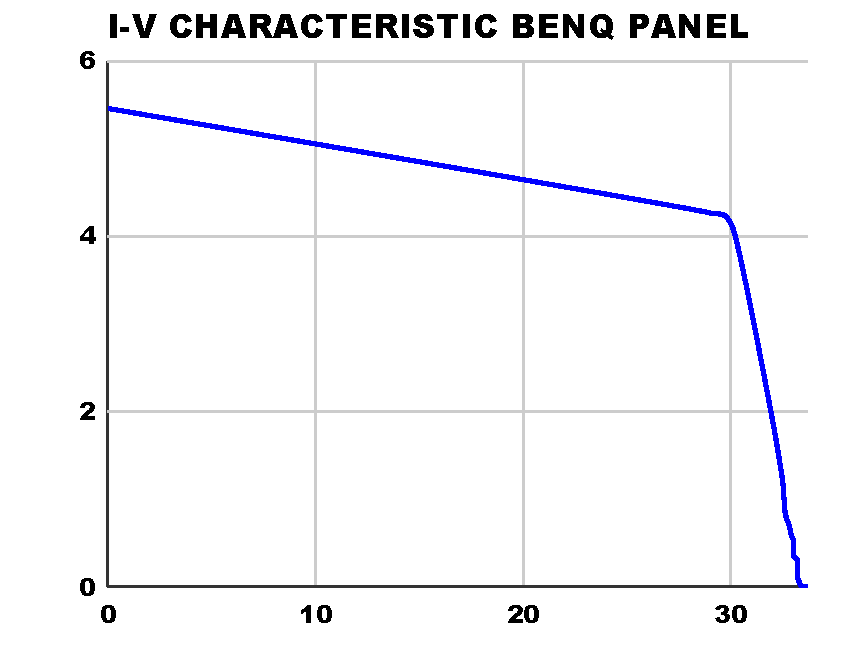
\includegraphics[scale=0.5]{benq-iv.pdf}
\subsection{Panda 60 cells}
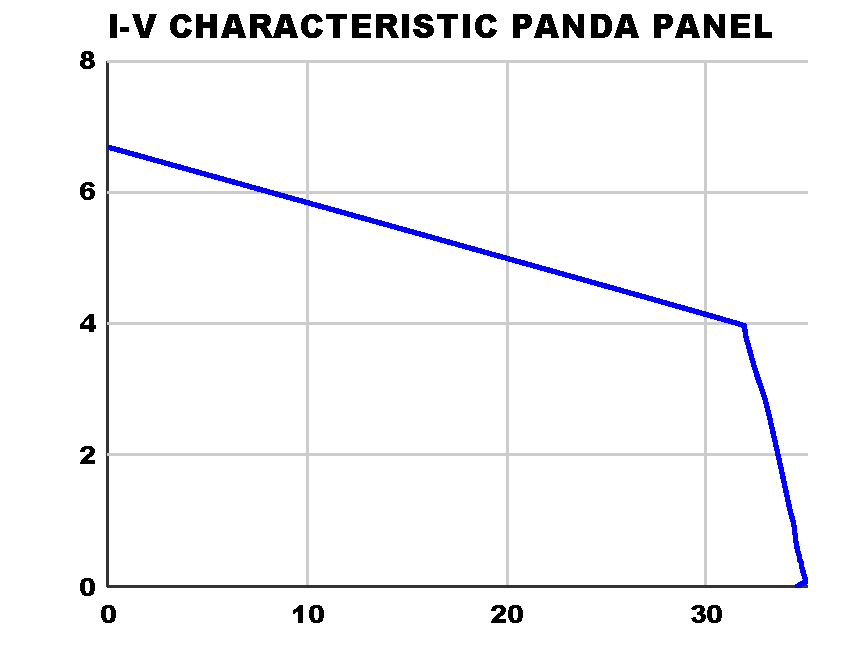
\includegraphics[scale=0.5]{panda-iv.pdf}

\subsection{Sharp NA-E135L5 series}
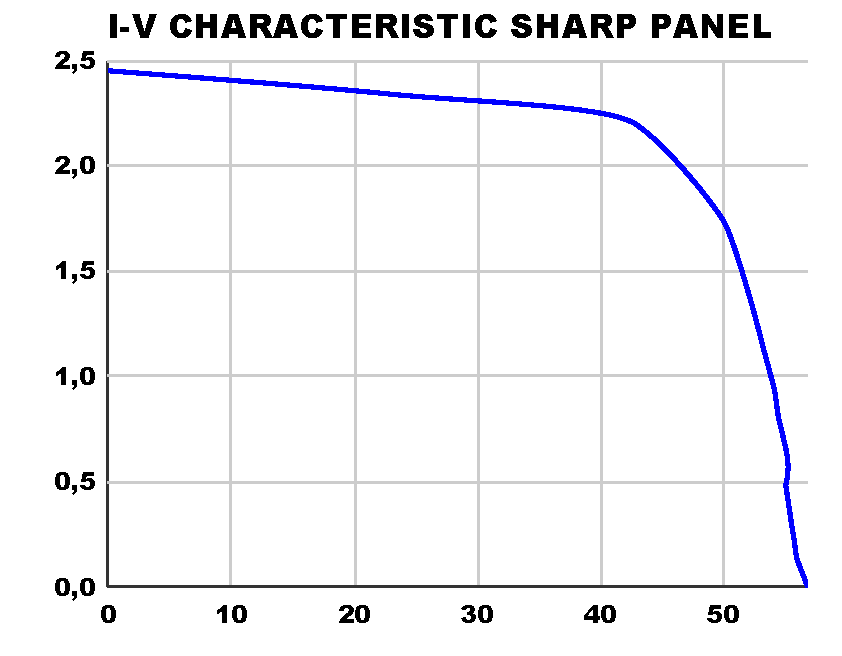
\includegraphics[scale=0.5]{sharp-iv.pdf}
%\begin{figure}[!ht]
%	\centering
%	\begin{subfigure}{0.7\textwidth}
%	  \centering
%	  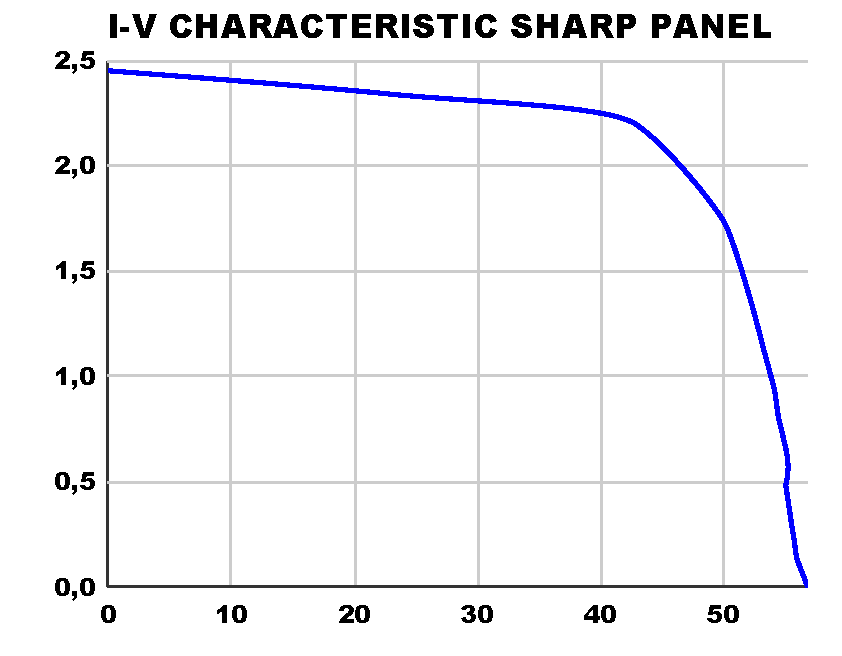
\includegraphics[width=.5\linewidth]{sharp-iv.pdf}
%	  \caption{Our graph}
%	  \label{fig:sub1}
%	\end{subfigure}%
%	\begin{subfigure}{.5\textwidth}
%	  \centering
%%	  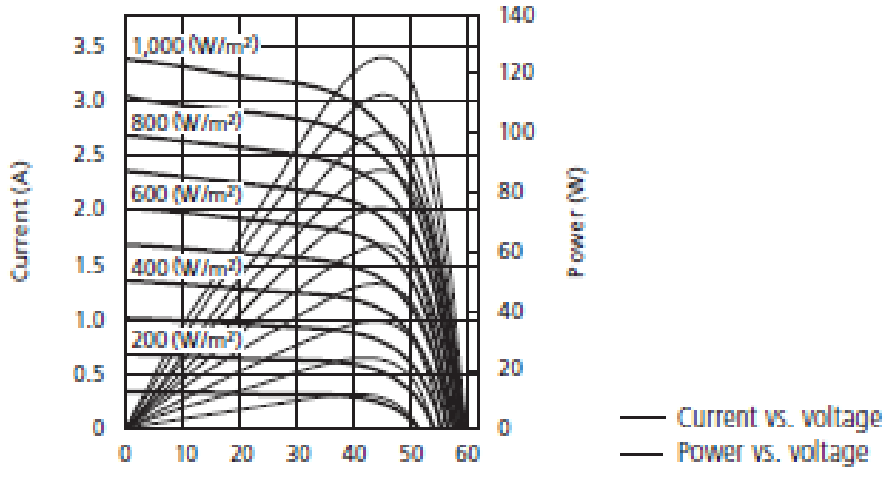
\includegraphics[width=.47\linewidth]{sharp-data-iv.png}
%	  \caption{Datasheet graph}
%	  \label{fig:sub2}
%	\end{subfigure}
%	\end{figure}

\section{Data analisys}
\subsection{Radiation}
Traced the graph we were able to hypothesize the amount of light that was reaching the panelr in other words 
the radiation.\\
We did this comparing our graphs with the datasheet's one that have multiple curves for different radiation
we used the maximum value of current for reference.\\
Only the graphs of the \textit{BenQ} and the \textit{Sharp} were provided, in both graphs our maximum current
was between the 800 $W/m^2$ and the 600 $W/m^2$ or 500 $W/m^2$ one, but it was surely closer to the 800 $W/m^2$
curve so after doing an approximate average we came to the conclusion that the radiation was 
\colorbox{Red}{750 $W/m^2$ or 720$W/m^2$} 
.\\


\section{Conclusions}

\end{document}